% Hlavicka pro protokoly z fyzikalniho praktika.
% Verze pro: LaTeX
% Verze hlavicky: 22. 2. 2007
% Autor: Ustav fyziky kondenzovanych latek
% Ke stazeni: www.physics.muni.cz/ufkl/Vyuka/
% Licence: volne k pouziti, nejlepe k vcasnemu odevzdani protokolu z Vaseho mereni.

\documentclass[a4paper,11pt]{article}

% Kodovani (cestiny) v dokumentu: utf-8
%\usepackage[cp1250]{inputenc}	% Omezena stredoevropska kodova stranka, pouze MSW.
\usepackage[utf8]{inputenc}	% Doporucujeme pouzivat UTF-8 (unicode).
\usepackage[T1]{fontenc}
\usepackage{lmodern}

%%% Nemente:
\usepackage[margin=2cm]{geometry}
\newtoks\jmenopraktika \newtoks\jmeno \newtoks\datum
\newtoks\obor \newtoks\skupina \newtoks\rocnik \newtoks\semestr
\newtoks\cisloulohy \newtoks\jmenoulohy
\newtoks\tlak \newtoks\teplota \newtoks\vlhkost
\usepackage{amsmath}
\usepackage{mathtools}
\usepackage{graphicx}
\usepackage{multirow}

\usepackage{pgfplotstable} 
\usepackage{booktabs}

\graphicspath{ {./images/} }
%%% Nemente - konec.


%%%%%%%%%%% Doplnte pozadovane polozky:

\jmenopraktika={Fyzikální praktikum 3}  % nahradte jmenem vaseho predmetu
\jmeno={Artem Gorodilov}            % nahradte jmenem mericiho
\datum={22. ~dubna  2024}        % nahradte datem mereni ulohy
\obor={Astrofyzika}                     % nahradte zkratkou vami studovaneho oboru
\skupina={Po 14:00}            % nahradte dobou vyuky vasi seminarni skupiny
\rocnik={II}                  % nahradte rocnikem, ve kterem studujete
\semestr={II}                 % nahradte semestrem, ve kterem studujete

\cisloulohy={H}               % nahradte cislem merene ulohy
\jmenoulohy={Studium činnosti fotonásobiče} % nahradte jmenem merene ulohy

\tlak={979}                   % nahradte tlakem pri mereni (v hPa)
\teplota={21.4}               % nahradte teplotou pri mereni (ve stupnich Celsia)
\vlhkost={46}               % nahradte vlhkosti vzduchu pri mereni (v %)

%%%%%%%%%%% Konec pozadovanych polozek.


%%%%%%%%%%% Uzitecne balicky:
\usepackage[czech]{babel}
\usepackage{graphicx}
\usepackage{amsmath}
\usepackage{xspace}
\usepackage{url}
\usepackage{indentfirst}
\usepackage{listings}
\usepackage{subcaption}
\usepackage{caption}
\usepackage{tabularx}
\usepackage[labelformat=parens,labelsep=quad,skip=3pt]{caption}
\captionsetup[figure]{name=Obrázek}

%%%%%% Zamezeni parchantu:
\widowpenalty 10000 \clubpenalty 10000 \displaywidowpenalty 10000
%%%%%% Parametry pro moznost vsazeni vetsiho poctu obrazku na stranku
\setcounter{topnumber}{3}	  % max. pocet floatu nahore (specifikace t)
\setcounter{bottomnumber}{3}	  % max. pocet floatu dole (specifikace b)
\setcounter{totalnumber}{6}	  % max. pocet floatu na strance celkem
\renewcommand\topfraction{0.9}	  % max podil stranky pro floaty nahore
\renewcommand\bottomfraction{0.9} % max podil stranky pro floaty dole
\renewcommand\textfraction{0.1}	  % min podil stranky, ktery musi obsahovat text
\intextsep=8mm \textfloatsep=8mm  %\intextsep pro ulozeni [h] floatu a \textfloatsep pro [b] or [t]

% Tecky za cisly sekci:
\renewcommand{\thesection}{\arabic{section}.}
\renewcommand{\thesubsection}{\thesection\arabic{subsection}.}
% Jednopismenna mezera mezi cislem a nazvem kapitoly:
\makeatletter \def\@seccntformat#1{\csname the#1\endcsname\hspace{1ex}} \makeatother

\begin{document}

\thispagestyle{empty}

{
\begin{center}
\sf 
{\Large Ústav fyzikální elektroniky PřF MU} \\
\bigskip
{\huge \bfseries FYZIKÁLNÍ PRAKTIKUM} \\
\bigskip
{\Large \the\jmenopraktika}
\end{center}

\bigskip

\sf
\noindent
\setlength{\arrayrulewidth}{1pt}
\begin{tabular*}{\textwidth}{@{\extracolsep{\fill}} l l}
\large {\bfseries Zpracoval:}  \the\jmeno & \large  {\bfseries Naměřeno:} \the\datum\\[2mm]
\large  {\bfseries Obor:} \the\obor  \hspace{40mm}  {\bfseries Skupina:} \the\skupina %
%{\bfseries Ročník:} \the\rocnik \hspace{5mm} {\bfseries Semestr:} \the\semestr  
&\large {\bfseries Testováno:}\\
\\
\hline
\end{tabular*}
}

\bigskip

{
\sf
\noindent \begin{tabular}{p{3cm} p{0.6\textwidth}}
\Large  Úloha č. {\bfseries \the\cisloulohy:} \par
\smallskip
% $T=\the\teplota$~$^\circ$C \par
% $p=\the\tlak$~hPa \par
% $\varphi=\the\vlhkost$~\%
&\Large \bfseries \the\jmenoulohy  \\[2mm]
\end{tabular}
}

\vskip10pt
    \begin{minipage}[t]{0.5\textwidth} 
        \section{Zadání}    
            \begin{enumerate}
                \item Stanovit závislost koeficientu sekundární emise na energii elektronů dopadajících na dynodu.
                \par Vynesti do grafu i závislost ln$(\sigma / U)$ = $f(U)$. 
                \par Zjistit, jestli koefcient sekundární emise $\sigma$
                závisí na intenzitě osvětlení fotokatody.

                \item Stanovit a vynést do grafu závislost integrální citlivosti fotonásobiče a zesílení fotonásobiče
                na napětí na násobiči $S$ = $f(U_a)$ a $M$ = $f(U_a)$.

                \item Stanovte integrální citlivost fotokatody $k$ = $I_f/\Phi$.
                
                \item Prověřit vliv temného proudu na přesnost měření.
            \end{enumerate}
        \section{Teorie}
                Fotonásobič je zařízení, které zesiluje slabé světelné signály. Skládá se z fotokatody, dynody (několik dyod) a anody. 
                \par Fotonásobič funguje na principu fotoelektrického jevu. Foton dopadající na fotokatodu vyvolá emisi elektronů. Tyto elektrony jsou urychlovány elektrickým polem k dynodám, kde se díky nárazové ionizaci uvolní další elektrony. Tyto elektrony jsou následně urychlovány k anodě, kde vzniká elektrický signál. Schema fotonásobiče je zobrazeno na obrázku (\ref{fig:scheme}).
                \par Sekundární emise je definována jako poměr proudů secundárních elektronů $I_{sec}$ a proudů primárních elektronů $I_{prim}$. V našem případě máme fotonásobič s dvěma dynodami, takže koeficient sekundární emise $\sigma$ je definován jako:
    \end{minipage}
    \hspace{10pt}
    \begin{minipage}[t]{0.5\textwidth} 
                \vspace{10pt}   
                \par \centering
                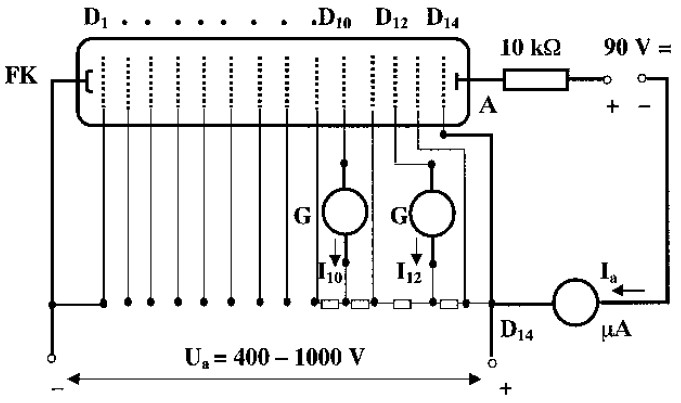
\includegraphics[scale=0.45]{scheme}
                \captionsetup{justification=centering, font=footnotesize}
                \captionof{figure}{Schéma elektrického zapojení fotonásobiče. Napětí na násobiči $U_a$ je rozděleno napět'ovým děličem a je přivedeno na jednotlivé dynody.}
                \label{fig:scheme}
                \vspace{10pt}
                \raggedright   

                \begin{equation}
                    \sigma = \sqrt{\frac{I_{12}}{I_{10}}}
                \end{equation}
                kde $I_{12}$ je proud na dvanácté dynodě a $I_{10}$ je proud na desáté dynodě. Odmocnina je zde proto, že mame dvě dynody.

                \par Celý postup zesílení elektronového toku z fotokatody lze zjednodušeně popsat následujícími vztahy. Proud elektronů z fotokatody $I_f$ závisí na světelném toku dopadajícím na fotokatodu podle Stoletovova zákona pro bílé světlo:
                \begin{equation}
                    I_f = k \Phi
                \end{equation}
                kde $k$ je integrální citlivost fotokatody a $\Phi$ je světelný tok.

                \par Známe li anodový proud $I_a$ a koficient sekundární emise $\sigma$, můžeme vypočítat proud elektronů na fotokatodě $I_f$:
                \begin{equation}
                    I_f = \frac{I_a}{\sigma^n}
                \end{equation}
                kde $n$ je počet dynod.
    \end{minipage}
\newpage
    \begin{minipage}[t]{0.5\textwidth} 
                \vspace{-50pt}
                \par Zesílení fotonásobiče $M$ je definováno jako poměr anodového proudu $I_a$ a fotokatodového proudu $I_f$:
                \begin{equation}
                    M = \frac{I_a}{I_f} = \sigma^n
                \end{equation}

                \par Integrální citlivost fotonásobiče $S$ je definována jako poměr anodového proudu $I_a$ a světelného toku $\Phi$:
                \begin{equation}
                    S = \frac{I_a}{\Phi} = Mk
                \end{equation}

        \section{Měření}
                K převodu dělení komory fotonásobiče na světelný proud jsme použili údaje o graduaci optického klínu. Vzali jsme hodnoty, které nám byly poskytnuty, a provedli fitování polynomem třetího stupně. Výsledky jsou uvedeny na obrázku (\ref{fig:grad}). 

                \vspace{10pt}   
                \par \centering
                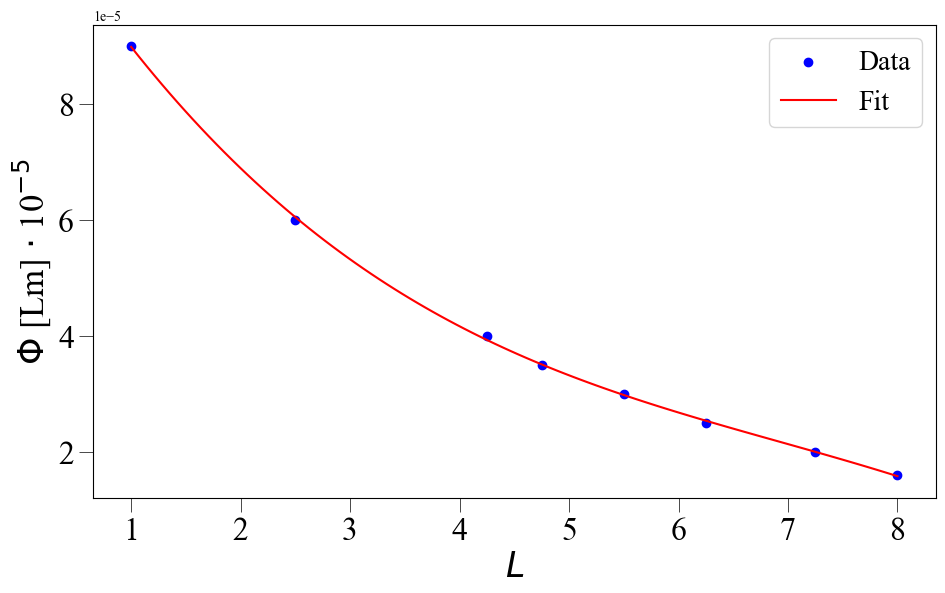
\includegraphics[scale=0.33]{grad}
                \captionsetup{justification=centering, font=footnotesize}
                \captionof{figure}{Gradace optického klínu.}
                \label{fig:grad}
                \vspace{10pt}
                \raggedright 

            \subsection{Temný proud}
                Jsme změřili temný proud $I_{10}$, $I_{12}$ a $I_a$ pro různé hodnoty napětí na násobiči $U_a$. Naměřené hodnoty jsou uvedeny v tabulce (1) a na obrázku (\ref{fig:dc}). Naměřené hodnoty jsme fitovali polynomem třetího stupně pro $I_a$, $I_{12}$ a lineární regresí pro $I_{10}$. Hodnoty fitů byly poté použity ke korekci naměřených dat použitých dale ve výpočtech.  

            \subsection{Sekundární emise}
                \par Poté jsme pomocí vzorce (1) zjistili koeficient sekundární emise $\sigma$ pro diody 10 a 12. Za tímto účelem jsme změřili hodnoty proudů $I_10$ a $I_12$ v závislosti na světelném proudu $\Phi$. Měření byla provedena pro anodové napětí:
                \begin{center}
                    $U_{a,1}$ = 730 [V] a $U_{a,2}$ = 704 [V]
                \end{center}
                \par Naměřené a vypočtené údaje jsou uvedeny v tabulkách (2) a (3).

                \par Získali jsme následující hodnoty koeficientů sekundárních emisí: 
                \begin{center}
                    $\sigma_{730 V}$ = 3.47(1) a $\sigma_{704 V}$ = 3.33(1)
                \end{center}
    
    \end{minipage}
    \hspace{10pt}
    \begin{minipage}[t]{0.5\textwidth} 
                \vspace{-50pt}
                \par \centering
                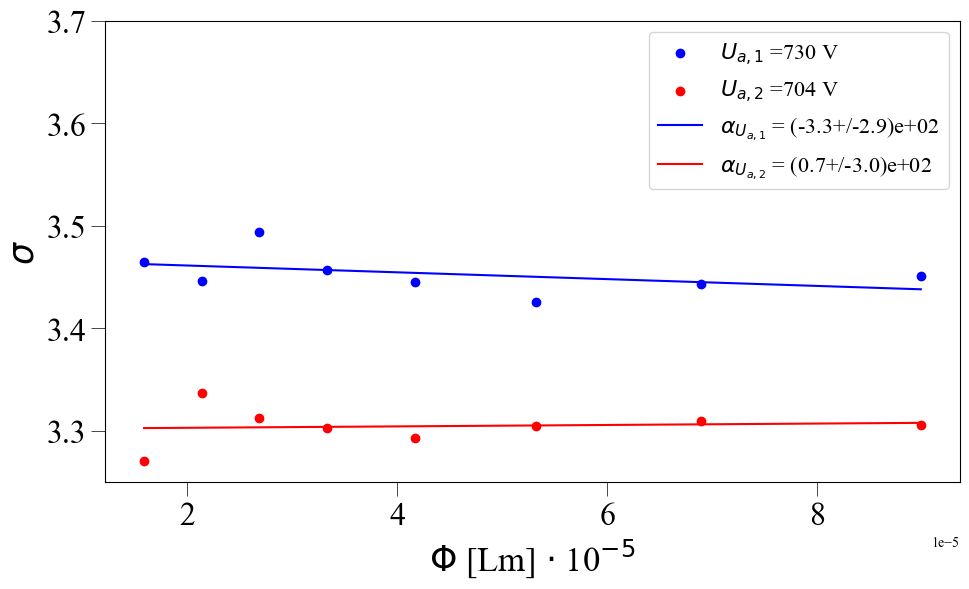
\includegraphics[scale=0.33]{sigma(F)}
                \captionsetup{justification=centering, font=footnotesize}
                \captionof{figure}{Závislost koeficientu sekundární emise na světelném proudu.}
                \label{fig:sigma(F)}
                \vspace{10pt}
                \raggedright 
                
                \par Abychom zjistili, zda existuje závislost koeficientu sekundární emise na světelném proudu, vynesli jsme graf (\ref{fig:sigma(F)}) závislosti $\sigma$ na $\Phi$.
                \par Jsme také provedli lineární fitování závislosti $\sigma$ = $f(\Phi)$ abychom zjistili stupeň závislosti.
            \subsection{Zesílení a integrální citlivost}
                Poté jsme provedli tři měření závislosti anodového proudu $I_a$ a proudů na diodách 10 a 12, $I_{10}$ a $I_{12}$ na anodovém napětí $U_a$. Byla provedena tři měření při třech hodnotách světelného proudu:
                \begin{center}
                    $\Phi_1$ = 8.98 $\cdot$ 10$^{-5}$ [Lm$\cdot$ 10$^{-5}$]
                    \par $\Phi_2$ = 4.17 $\cdot$ 10$^{-6}$ [Lm$\cdot$ 10$^{-5}$]
                    \par $\Phi_3$ = 2.14 $\cdot$ 10$^{-5}$ [Lm$\cdot$ 10$^{-5}$]
                \end{center}
                \par Podle vzorce (1) jsme vypočítali koeficient sekundární emise $\sigma$ pro diody 10 a 12. Dale umcnením koeficientu sekundární emise $\sigma$ na druhou jsme získali zesílení fotonásobiče $M$ a pak, podle vzorce (4) jsme vypočítali proud elektronů na fotokatodě $I_f$. Odsud pomocí vzorce (2) jsme vypočítali integrální citlivost fotokatody $k$. Pak jsme byly schopni vypočítat integrální citlivost fotonásobiče $S$ podle vzorce (5). Naměřené a vypočtené hodnoty jsou uvedeny v tabulkách (4), (5) a (6). Vynesli jsme do grafu (\ref{fig:ln(sigma)}) zavislost ln$(\sigma / U)$ = $f(U)$ pro všechny tři hodnot. Pak vynesli jsme grafy (\ref{fig:S(U)}) a (\ref{fig:M(U)}) závislostí $S$ a $M$ na $U_a$ pro všechny tři hodnoty světelného proudu $\Phi$.
                
                \vspace{10pt}   
                \par \centering
                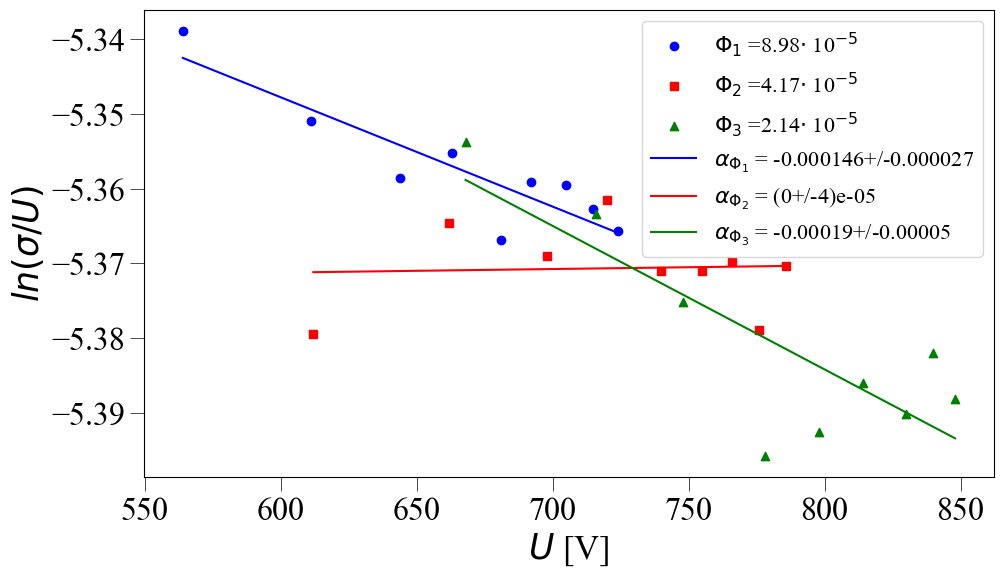
\includegraphics[scale=0.33]{ln(sigma)}
                \captionsetup{justification=centering, font=footnotesize}
                \captionof{figure}{Závislost ln$(\sigma / U)$ = $f(U)$.}
                \label{fig:ln(sigma)}
                \vspace{10pt}
                \raggedright 

    \end{minipage}
\newpage
    \begin{minipage}[t]{0.5\textwidth}
                \vspace{0pt}   
                \par \centering
                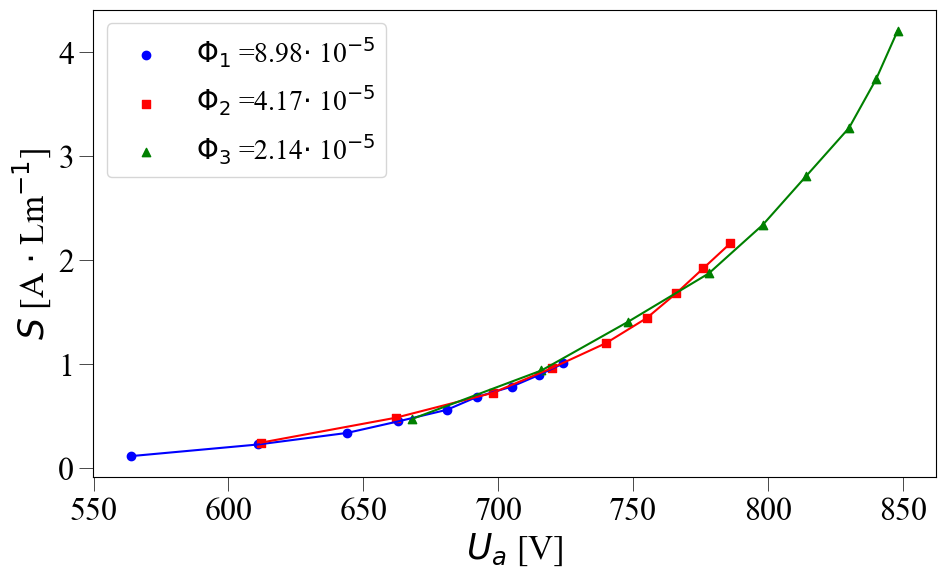
\includegraphics[scale=0.33]{S(U)}
                \captionsetup{justification=centering, font=footnotesize}
                \captionof{figure}{Závislost integrální citlivosti fotonásobiče na napětí na násobiči $S$ = $f(U_a)$.}
                \label{fig:S(U)}
                \vspace{10pt}
                \raggedright 

                \vspace{0pt}   
                \par \centering
                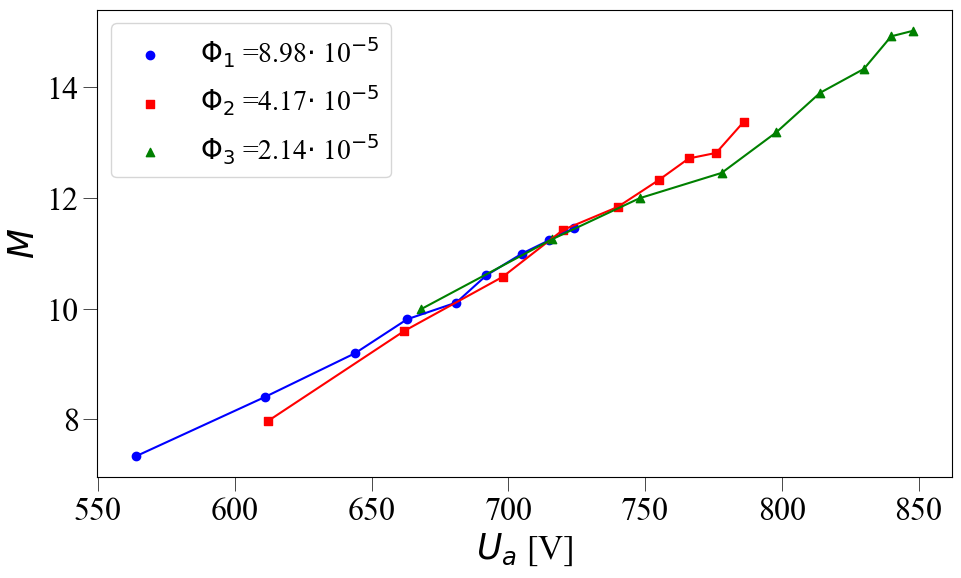
\includegraphics[scale=0.33]{M(U)}
                \captionsetup{justification=centering, font=footnotesize}
                \captionof{figure}{Závislost zesílení fotonásobiče na napětí na násobiči $M$ = $f(U_a)$.}
                \label{fig:M(U)}
                \vspace{10pt}
                \raggedright 
    \end{minipage}
    \begin{minipage}[t]{0.5\textwidth}
                \vspace{0pt}   
                \par \centering
                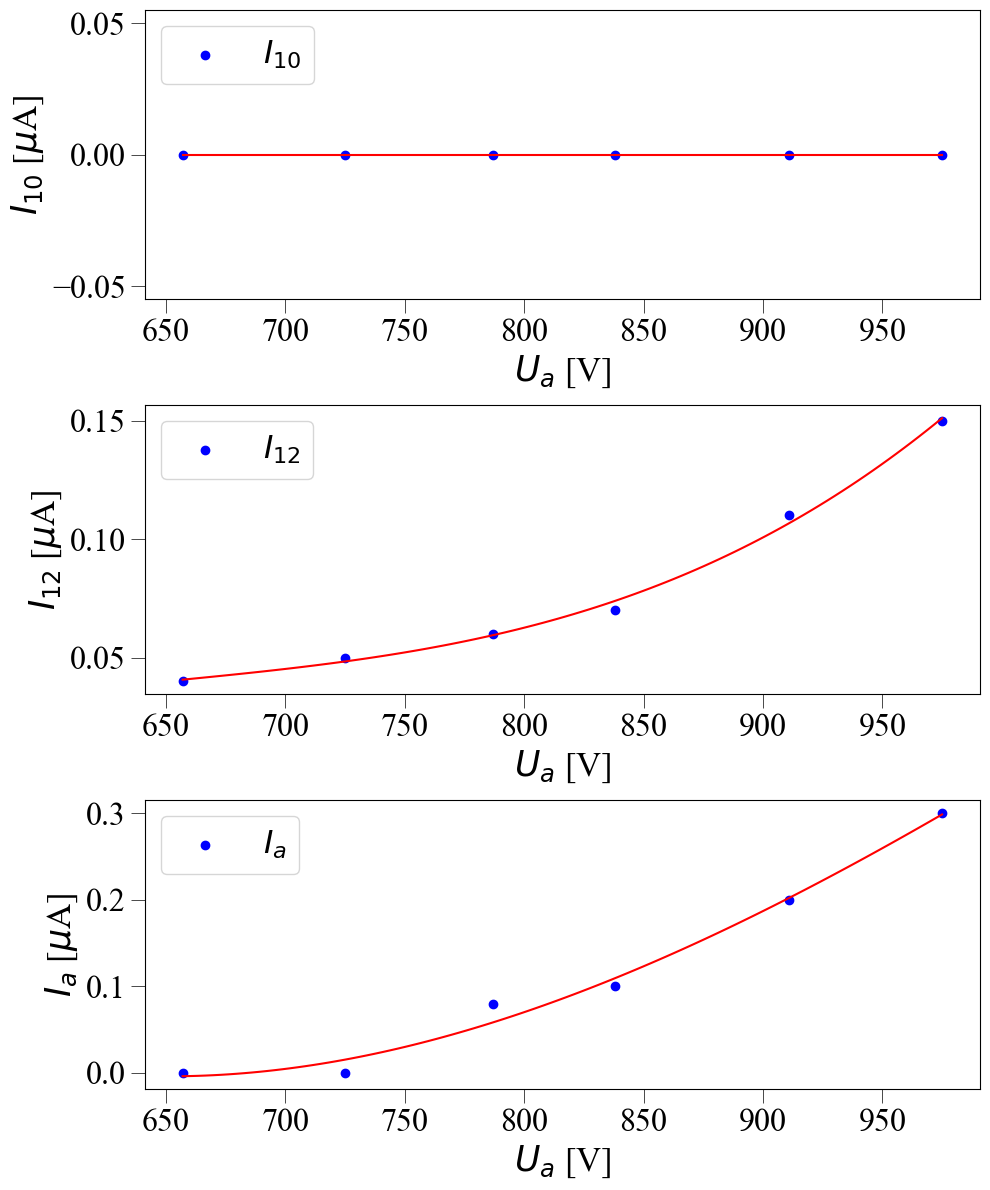
\includegraphics[scale=0.33]{dc}
                \captionsetup{justification=centering, font=footnotesize}
                \captionof{figure}{Závislost temného proudu na napětí na násobiči.}
                \label{fig:dc}
                \vspace{10pt}
                \raggedright 
    \end{minipage}
                \vspace{10pt}
                \par K výpočtu veličin a jejich nejistot byla použita knihovna Uncertinties pro Python \cite{uncertainties}. Chyby byly rozšířeny o Studentův koeficient (2-Tail Confidence Level) s ohledem na stupně volnosti pro každou hodnotu, pro interval spolehlivosti 68.27\%.
        \section{Závěr} 
                Byla zjištěna závislost koeficientu sekundární emise $\sigma$ na světelném proudu $\Phi$. Z grafu (\ref{fig:sigma(F)}) bylo zjištěno, že koeficient sekundární emise $\sigma$ slabo závisí na světelném proudu $\Phi$. Z grafu je patrné, že sklon přímky lze v rámci chyby fitování považovat za nulový $\alpha_{U_{a,1}}$ = -(330 $\pm$ 290) [Lm$^{-1}$], $\alpha_{U_{a,2}}$ = -(70 $\pm$ 300) [Lm$^{-1}$]. To je patrné zejména při hodnotách světelného proudu $\Phi$ > 3 $\cdot$ 10$^{-5}$ [Lm$\cdot$ 10$^{-5}$]. Při $\Phi$ < 3 $\cdot$ 10$^{-5}$ [Lm$\cdot$ 10$^{-5}$] dochází ke skokům v hodnotách $\sigma$, které mohou být způsobeny nepřesností měření proudu na desáté diodě $I_{10}$, protože při nízkých hodnotách $\Phi$ nabývá $I_{10}$ poměrně malých hodnot. 

                \vspace{5pt}
                \par Ze zavislosti ln$(\sigma / U)$ = $f(U)$ vyplývá, že hodnota ln$(\sigma / U)$ s rostoucím napětím lineárně klesá. To je dobře vidět zejména pro $\Phi_1$ a $\Phi_3$. U $\Phi_2$ je klesající trend menší, což může být způsobeno nepřesností měření. 
                
                \vspace{5pt}
                \par Z grafu (\ref{fig:S(U)}) závislosti $S$ na $U_a$ je vidět, že integrální citlivost fotonásobiče $S$ s rostoucím napětím roste exponenciálně. 

                \vspace{5pt}
                \par Z grafu (\ref{fig:M(U)}) závislosti $M$ na $U_a$ je vidět, že zesílení fotonásobiče $M$ s rostoucím napětím roste spíše lineárně.

                \vspace{5pt}
                \par Z tabulky (6) je patrné, že temný proud začíná být patrný při napětí $U_a$ > 800 V.

                \renewcommand{\refname}{Odkazy}
                \begin{thebibliography}{9}
                    \bibitem{uncertainties}
                        Uncertainties, Dostupné online: \url{https://pypi.org/project/uncertainties}
                \end{thebibliography} 

    \begin{center}
        \section{Appendix}
            \begin{center}
                \subsection{Tabulka naměřených hodnot pro temný proud}
                    \pgfplotstabletypeset[
                        col sep=comma, % Defines the separator, comma for CSV
                        string type, % Treats columns as strings (not math mode)
                        every head row/.style={before row=\toprule,after row=\midrule},
                        every last row/.style={after row=\bottomrule},
                        columns/U_a/.style={column name=$U_a$ [V]},
                        columns/I_a/.style={column name=$I_a$ [$\mu$A]},
                        columns/I_10/.style={column name=$I_{10}$ [$\mu$A]},
                        columns/I_12/.style={column name=$I_{12}$ [$\mu$A]},
                        ]{data/DC_out.csv}
            \end{center}

            \subsection{Tabulka naměřených a vypočtených hodnot pro $U_{a,1}$ = 730 V}
                \pgfplotstabletypeset[
                col sep=comma, % Defines the separator, comma for CSV
                string type, % Treats columns as strings (not math mode)
                every head row/.style={before row=\toprule,after row=\midrule},
                every last row/.style={after row=\bottomrule},
                columns/F/.style={column name=$\Phi$ [Lm$\cdot$ 10$^{-5}$]},
                columns/I_a/.style={column name=$I_a$ [$\mu$A]},
                columns/I_10/.style={column name=$I_{10}$ [$\mu$A]},
                columns/I_12/.style={column name=$I_{12}$ [$\mu$A]},
                columns/sigma/.style={column name=$\sigma$}
                ]{data/U_1_out.csv}
    \end{center}
    \begin{center}
        \subsection{Tabulka naměřených hodnot pro $U_{a,2}$ = 704 V}
            \pgfplotstabletypeset[
                col sep=comma, % Defines the separator, comma for CSV
                string type, % Treats columns as strings (not math mode)
                every head row/.style={before row=\toprule,after row=\midrule},
                every last row/.style={after row=\bottomrule},
                columns/F/.style={column name=$\Phi$ [Lm$\cdot$ 10$^{-5}$]},
                columns/I_a/.style={column name=$I_a$ [$\mu$A]},
                columns/I_10/.style={column name=$I_{10}$ [$\mu$A]},
                columns/I_12/.style={column name=$I_{12}$ [$\mu$A]},
                columns/sigma/.style={column name=$\sigma$}
                ]{data/U_2_out.csv}
    \end{center}

    \begin{center}
        \subsection{Tabulka naměřených hodnot pro $\Phi_1$ = 8.98 $\cdot$ 10$^{-5}$ [Lm$\cdot$ 10$^{-5}$]}
            \pgfplotstabletypeset[
                col sep=comma, % Defines the separator, comma for CSV
                string type, % Treats columns as strings (not math mode)
                every head row/.style={before row=\toprule,after row=\midrule},
                every last row/.style={after row=\bottomrule},
                columns/U_a/.style={column name=$U_a$ [V]},
                columns/I_a/.style={column name=$I_a$ [$\mu$A]},
                columns/I_10/.style={column name=$I_{10}$ [$\mu$A]},
                columns/I_12/.style={column name=$I_{12}$ [$\mu$A]},
                columns/sigma/.style={column name=$\sigma$},
                columns/M/.style={column name=$M$},
                columns/S/.style={column name=$S$ [A $\cdot$ Lm$^{-1}$]},
                columns/I_f/.style={column name=$I_f$ [$\mu$A]},
                columns/k/.style={column name=$k$ [$\cdot$ Lm$^{-1}$]},
                columns/ln(sig/V)/.style={column name=ln$(\sigma / U)$}
                ]{data/F_1_out.csv}
    \end{center}

    \begin{center}
        \subsection{Tabulka naměřených hodnot pro $\Phi_2$ = 4.17 $\cdot$ 10$^{-6}$ [Lm$\cdot$ 10$^{-5}$]}
            \pgfplotstabletypeset[
                col sep=comma, % Defines the separator, comma for CSV
                string type, % Treats columns as strings (not math mode)
                every head row/.style={before row=\toprule,after row=\midrule},
                every last row/.style={after row=\bottomrule},
                columns/U_a/.style={column name=$U_a$ [V]},
                columns/I_a/.style={column name=$I_a$ [$\mu$A]},
                columns/I_10/.style={column name=$I_{10}$ [$\mu$A]},
                columns/I_12/.style={column name=$I_{12}$ [$\mu$A]},
                columns/sigma/.style={column name=$\sigma$},
                columns/M/.style={column name=$M$},
                columns/S/.style={column name=$S$ [A $\cdot$ Lm$^{-1}$]},
                columns/I_f/.style={column name=$I_f$ [$\mu$A]},
                columns/k/.style={column name=$k$ [$\cdot$ Lm$^{-1}$]},
                columns/ln(sig/V)/.style={column name=ln$(\sigma / U)$}
                ]{data/F_2_out.csv}
    \end{center}

    \begin{center}
        \subsection{Tabulka naměřených hodnot pro $\Phi_3$ = 2.14 $\cdot$ 10$^{-5}$ [Lm$\cdot$ 10$^{-5}$]}
            \pgfplotstabletypeset[
                col sep=comma, % Defines the separator, comma for CSV
                string type, % Treats columns as strings (not math mode)
                every head row/.style={before row=\toprule,after row=\midrule},
                every last row/.style={after row=\bottomrule},
                columns/U_a/.style={column name=$U_a$ [V]},
                columns/I_a/.style={column name=$I_a$ [$\mu$A]},
                columns/I_10/.style={column name=$I_{10}$ [$\mu$A]},
                columns/I_12/.style={column name=$I_{12}$ [$\mu$A]},
                columns/sigma/.style={column name=$\sigma$},
                columns/M/.style={column name=$M$},
                columns/S/.style={column name=$S$ [A $\cdot$ Lm$^{-1}$]},
                columns/I_f/.style={column name=$I_f$ [$\mu$A]},
                columns/k/.style={column name=$k$ [$\cdot$ Lm$^{-1}$]},
                columns/ln(sig/V)/.style={column name=ln$(\sigma / U)$}
                ]{data/F_3_out.csv}
    \end{center}
\end{document}